\section{Methodology}
\label{sec:method}

To overcome the limitations that a single path planner cannot optimize the visiting order and that an unconstrained traveling salesman model ignores obstacle-induced cost, this section presents a heuristic cooperative framework consisting of two stages. Hyperparameters used in the algorithms of this section are denoted symbolically; their default values, unless otherwise stated, are listed in Table~\textcolor{blue}{\ref{tab:params}}. Specifically, the first stage employs the improved A* global planner proposed in this paper to search for collision-free point-to-point shortest paths on a grid map, and produces high-quality continuous paths through safety-distance-aware path simplification and cubic spline smoothing. The second stage takes the cost matrix produced by the first stage as input and uses the proposed MMAS-VND-CL ant colony optimization solver to determine the optimal visiting sequence of multiple goal points. The two stages are coupled through the cost matrix, jointly completing the full pipeline from geometric routing to combinatorial ordering. Section~\textcolor{blue}{\ref{subsec:jps}} and Section~\textcolor{blue}{\ref{subsec:post}} present the global path planner and its post-processing, Section~\textcolor{blue}{\ref{subsec:aco}} details the open traveling salesman solver, and Section~\textcolor{blue}{\ref{subsec:coop}} describes the overall design of the two-layer cooperative framework.

\subsection{Improved A* Global Path Planner}
\label{subsec:jps}

\subsubsection{Jump Point Search}

Conventional A* expands neighbors cell by cell; in large open regions the number of expanded nodes grows in proportion to the map area. To address this issue, this paper adopts an improved A* algorithm based on Jump Point Search (JPS)~\textcolor{blue}{\cite{ref11,ref12}}. JPS exploits grid symmetry to prune neighbors: along the expansion direction, only natural neighbors and forced neighbors induced by obstacles are retained. The jump function $\mathrm{jump}(r, c, dr, dc)$ advances along a given direction until the goal is reached, an obstacle is encountered, or a forced neighbor is discovered; intermediate nodes are not inserted into the open set. Jump-point costs are accumulated using Manhattan or diagonal distance. After the search completes, the path is recovered by backtracking parent pointers and completing straight-line interpolation between adjacent jump points. The pruning rules are illustrated in Fig.~\textcolor{blue}{\ref{fig:jps_pruning}}. On this basis, three improvements are made in this paper.

\begin{figure}[!t]
\centering
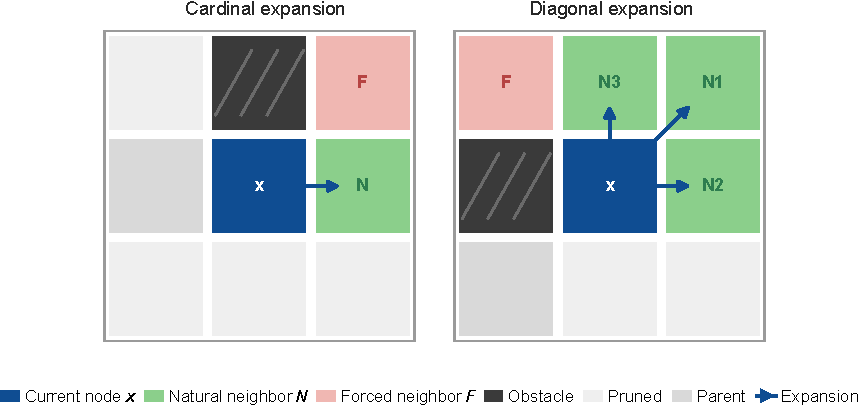
\includegraphics[width=3.0in]{figures/jps_pruning}
\caption{Illustration of the JPS neighbor-pruning rules.}
\label{fig:jps_pruning}
\end{figure}

Owing to the jumping nature of JPS, diagonal moves in the reconstructed path may cut across obstacle corners. To address this issue, a diagonal corner-correction mechanism is introduced during path reconstruction: when a diagonal move is detected to pass through an obstacle corner, it is replaced by an L-shaped path along the grid boundary (row first and then column, or column first and then row), thereby avoiding collisions with obstacles. The corrected path follows grid boundaries strictly, which guarantees path feasibility.

Moreover, the pruning rules of JPS rely on a uniform grid structure. On maps with complex obstacle distributions, forced neighbors arise more frequently, the advantage of JPS is weakened, and in extreme cases the symmetry assumption may fail and cause the JPS search to fail. Therefore, the improved A* algorithm proposed in this paper automatically falls back to conventional A* and restarts the search when JPS exhausts the open set without finding a path, thus ensuring that a path is always found whenever a feasible solution exists. This degradation mechanism guarantees the robustness of the algorithm and enables it to adapt to environments of varying complexity.

\subsubsection{Tie-Breaking Strategy}

When multiple nodes in the open set share the same $f$-value, the selection order of standard A* depends on the specific implementation (typically first-in-first-out or random) and is essentially arbitrary. However, among nodes with identical $f$-values, a node with a smaller $h$-value has a larger actual cost $g = f - h$, i.e., it lies farther from the start and closer to the goal. Expanding such nodes first steers the search toward the goal without affecting the optimality guarantee. Accordingly, the improved A* algorithm adopts the tie-breaking rule ``when $f$-values are equal, prefer the node with the smaller $h$-value.'' The comparison rule between nodes in the binary heap is defined as
\begin{equation}
\begin{cases}
n_1, & f(n_1) < f(n_2) \\
n_2, & f(n_1) > f(n_2) \\
n_1, & f(n_1) = f(n_2) \land h(n_1) < h(n_2) \\
n_2, & f(n_1) = f(n_2) \land h(n_1) > h(n_2)
\end{cases}
\label{eq:tbreak}
\end{equation}
This comparison rule is embedded directly into the bubble-up (\texttt{bubbleUp}) and bubble-down (\texttt{bubbleDown}) operations of the binary heap.

From a physical standpoint, the evaluation function $f(n) = g(n) + h(n)$ implies that when two nodes share the same $f$-value, the one with the larger $g$ has the smaller $h$. A larger $g$ means the node is farther from the start, whereas a smaller $h$ means it is closer to the goal. Prioritizing such nodes biases the search toward the goal and reduces ineffective exploration in regions away from the goal. Since $h$ is already computed when a node is expanded, this tie-breaking strategy incurs no additional computational overhead.

\subsection{Path Post-Processing}
\label{subsec:post}

The path produced by JPS consists of a sequence of grid-center points and suffers from two major issues: it contains redundant intermediate points, and it is composed of discrete horizontal and vertical segments that lack smoothness. This section proposes a two-stage post-processing pipeline to resolve these problems.

\subsubsection{Safety-Aware Path Simplification}

Conventional path-simplification methods (e.g., corner pruning) directly connect non-adjacent nodes on the path and skip intermediate points to reduce the number of path points. However, such methods typically only check whether the connecting segment intersects obstacles and ignore the safety margin between path points and obstacles; in obstacle-dense regions this may yield paths that pass excessively close to obstacles. To address this issue, a safety-distance-aware path-simplification algorithm is proposed, whose core idea is to maintain a minimum safety distance between the path and obstacles during simplification.

The algorithm processes the input path in four steps.

First, the nodes at which the path direction changes are identified. For each intermediate node of the path, the directions of the segments connecting it to its predecessor and successor are computed. If the incoming and outgoing directions differ, the node is marked as a corner point. The start and end points of the path are always retained.

Second, starting from the current corner $C_i$, all subsequent corners $C_j$ ($j > i$) are scanned forward, and \textsc{IsLineFree} is invoked to verify that the segment $C_i \to C_j$ satisfies the safety-distance constraint. The \textbf{farthest} reachable corner $j^{*}$ is recorded. This corner becomes the new anchor, and all corners in between are skipped. This greedy strategy maximizes the single-step simplification while preserving safety.

Third, after the greedy step determines the farthest reachable corner $j^{*}$, the algorithm checks whether a skipped corner $k$ ($i < k < j^{*}$) can reach a farther corner $j'$ ($j' > j^{*}$) by a safety-compliant segment. For every pair $(k, j')$ that satisfies the safety constraint, the costs of the two resulting paths are computed and compared. If such an intermediate corner exists, a simplified path shorter than that of pure greedy may be obtained.

Fourth, the lengths of the two candidate paths are compared: Path~A (greedy) has length $d(C_i, C_{j^{*}}) + d(C_{j^{*}}, C_{j'})$, i.e., first reaching $j^{*}$ and then continuing to $j'$; Path~B (via the intermediate corner) has length $d(C_i, C_k) + d(C_k, C_{j'})$, i.e., bypassing $j^{*}$ and routing through $k$. If Path~B is shorter, the intermediate corner $C_k$ is retained; otherwise, only the greedy result $C_{j^{*}}$ is kept. This comparison ensures that intermediate-corner exploration does not sacrifice path efficiency.

The safety-check function $\textsc{IsLineFree}(p_1, p_2, \mathrm{map}, d_{\mathrm{safe}})$ is implemented by dense sampling along the segment: sample points are densely drawn from $p_1$ to $p_2$ along the segment, and for each sample point its distance to the nearest obstacle-cell boundary is computed. If the distance of any sample point is smaller than the safety threshold $d_{\mathrm{safe}}$, the connection is deemed unsafe. The distance from a point to a cell boundary is given by
\begin{equation}
\begin{split}
d_x &= \max\left(0,\; |x_p - x_c| - 0.5\right)\\
d_y &= \max\left(0,\; |y_p - y_c| - 0.5\right)
\end{split}
\label{eq:dxymax}
\end{equation}

\begin{equation}
d(p, \mathrm{cell}) = \sqrt{d_x^2 + d_y^2}
\label{eq:dist}
\end{equation}
where $p = (x_p, y_p)$ is the sample point under the grid-to-continuous coordinate mapping described above, $(x_c, y_c)$ is the center of the obstacle cell, and the cell occupies the rectangular region $[x_c - 0.5, x_c + 0.5] \times [y_c - 0.5, y_c + 0.5]$. The $\max(0, \cdot)$ operator handles the case in which the sample point already falls within the horizontal or vertical extent of the cell along a given axis. When $d(p, \mathrm{cell}) < d_{\mathrm{safe}}$, the sample point has entered the safety exclusion zone of the obstacle cell. The safety-distance threshold $d_{\mathrm{safe}}$ is taken as the sum of the robot radius $r_{\mathrm{robot}}$ and an additional safety margin, thereby ensuring that the clearance from the path centerline to obstacles is no less than the robot radius and that collisions are avoided. Algorithm~\textcolor{blue}{\ref{alg:simplify}} gives the pseudocode of the path-simplification algorithm.

\begin{algorithm}[!t]
\caption{Safety-distance-aware path simplification}
\label{alg:simplify}
\begin{spacing}{0.9}
\begin{algorithmic}[1]
\REQUIRE grid path $P = [P_1, \ldots, P_N]$, occupancy grid, safety margin $d_{\mathrm{safe}}$
\ENSURE simplified path $P_s$ ($|P_s| \leq N$)
\STATE $C \gets$ the corner points of $P$ where the direction changes, plus the two endpoints;
\STATE $P_s \gets [C_1]$; $\; i \gets 1$;
\WHILE{$i < |C|$}
\STATE $j^{*} \gets$ the farthest corner reachable from $C_i$ by a collision-free segment; \quad\textit{greedy forward scan}
\IF{$j^{*} = |C|$}
\STATE append $C_{|C|}$ to $P_s$ and break;
\ENDIF
\STATE $(k^{*}, j') \gets$ among all skipped corners $k$ ($i < k < j^{*}$) and farther corners $j$ ($j^{*} < j \leq |C|$), the pair with the largest $j$ such that the segment $C_k \to C_j$ is collision-free;
\IF{$k^{*}$ exists and $d(C_i, C_{k^{*}}) + d(C_{k^{*}}, C_{j'}) < d(C_i, C_{j^{*}}) + d(C_{j^{*}}, C_{j'})$}
\STATE append $C_{k^{*}}$ and $C_{j'}$ to $P_s$, and set $i \gets j'$; \quad\textit{route through the intermediate corner}
\ELSE
\STATE append $C_{j^{*}}$ to $P_s$, and set $i \gets j^{*}$;
\ENDIF
\ENDWHILE
\RETURN $P_s$;
\end{algorithmic}
\end{spacing}
\end{algorithm}

The pseudocode of the safety-check function \textsc{IsLineFree} is given in Algorithm~\textcolor{blue}{\ref{alg:islinefree}}. The search radius $d_{\max}$ is set to $\lceil d_{\mathrm{safe}} + 0.5 \rceil$, because cells beyond this distance cannot intersect the safety distance of any sample point.

\begin{algorithm}[!t]
\caption{IsLineFree }
\label{alg:islinefree}
\begin{spacing}{0.9}
\begin{algorithmic}[1]
\REQUIRE segment endpoints $p_1$, $p_2$ (grid coordinates), occupancy grid, safety margin $d_{\mathrm{safe}}$
\ENSURE true if the segment keeps distance $\geq d_{\mathrm{safe}}$ from every obstacle, false otherwise
\STATE $\ell \gets \max(|p_1.r - p_2.r|,\; |p_1.c - p_2.c|)$;
\STATE $N_s \gets \max(\lceil 10 \cdot \ell \rceil, 30)$; \quad\textit{number of dense sample points}
\STATE $d_{\max} \gets \lceil d_{\mathrm{safe}} + 0.5 \rceil$; \quad\textit{search radius in cells}
\FOR{$k = 0$ to $N_s$}
\STATE $p \gets p_1 + (k / N_s) \cdot (p_2 - p_1)$; \quad\textit{sample point in continuous coordinates}
\FOR{each cell $(r, c)$ within Chebyshev distance $d_{\max}$ of $p$}
\IF{$(r, c)$ is occupied}
\STATE $d \gets$ the distance from $p$ to the boundary of cell $(r, c)$; \quad\textit{see Eq.~\textcolor{blue}{\eqref{eq:dist}}}
\IF{$d < d_{\mathrm{safe}}$}
\STATE \RETURN false;
\ENDIF
\ENDIF
\ENDFOR
\ENDFOR
\RETURN true;
\end{algorithmic}
\end{spacing}
\end{algorithm}

\subsubsection{Arc-Length Parameterized Cubic Spline Smoothing}

Although the simplified path has removed redundant points, it is still composed of straight-line segments with curvature discontinuities at the corner points, and is therefore unsuitable for the smooth motion of an omnidirectional robot. This paper adopts arc-length parameterized cubic spline smoothing, using the cumulative Euclidean distance between path points rather than the point index as the parameter, so that the parameter space remains consistent with the actual geometric space. The smoothing process consists of three steps.

The first step is densification of sparse segments: segments whose adjacent points are separated by more than two grid units are detected. For these sparse segments, $\lfloor \ell / 2 \rfloor$ intermediate points are linearly interpolated along the segment between the two endpoints. The purpose of densification is to provide the spline with sufficient control points and to prevent spline overshoot (the Runge phenomenon) on long straight segments caused by an insufficient number of control points, which would otherwise cause the curve to deviate from the intended polyline or even clip obstacle corners.

The second step is arc-length parameterization. Let the densified path-point sequence be $\{P_0, P_1, \ldots, P_M\}$, where $P_i = (x_i, y_i)$ are continuous coordinates. The cumulative chord-length (arc-length) parameters are computed as $s_0 = 0$ and $s_i = s_{i-1} + \|P_i - P_{i-1}\|_2$ ($i = 1, 2, \ldots, M$). Cubic spline interpolation is then performed for $x(s)$ and $y(s)$ separately with $s$ as the independent variable, yielding the parametric curve $(x(s), y(s))$. On each subinterval $[s_i, s_{i+1}]$, the cubic spline is a cubic polynomial that guarantees continuity of the first- and second-order derivatives, and hence continuity of the curve curvature.

The third step is equal arc-length resampling. The final smoothed path-point sequence is generated by uniformly sampling along the arc-length parameter $s$ at an interpolation density $\rho$. Because $s$ is approximately linearly related to the actual geometric distance, equal arc-length sampling ensures a uniform spatial distribution of path points and avoids the problem of conventional equal-parameter sampling, which places points densely at high curvature and sparsely at low curvature. Algorithm~\textcolor{blue}{\ref{alg:smooth}} gives the pseudocode of the smoothing algorithm.

\begin{algorithm}[!t]
\caption{Arc-length parameterized cubic spline smoothing}
\label{alg:smooth}
\begin{spacing}{0.9}
\begin{algorithmic}[1]
\REQUIRE grid path $P = [P_1, \ldots, P_N]$, density $\rho$ (default $10$)
\ENSURE smoothed continuous path $Q = [Q_1, \ldots, Q_M]$ in $[x, y]$
\STATE convert each grid point $P_i = (r_i, c_i)$ to continuous coordinates $(x_i, y_i) = (c_i - 0.5,\; r_i - 0.5)$;
\FOR{each consecutive pair whose segment length exceeds $2$}
\STATE insert $\lfloor \mathrm{length} / 2 \rfloor$ equally spaced intermediate points along the segment; \quad\textit{densification to prevent spline overshoot}
\ENDFOR
\STATE compute the cumulative chord length $t_1 = 0$, $t_i = t_{i-1} + \|P_i - P_{i-1}\|_2$; \quad\textit{arc-length parameter}
\STATE remove duplicate $t$ values to keep strict monotonicity;
\STATE fit cubic splines $x(t)$ and $y(t)$ through the densified points;
\STATE sample $x(t)$ and $y(t)$ at $\rho$ points per segment to obtain $Q$;
\RETURN $Q$;
\end{algorithmic}
\end{spacing}
\end{algorithm}

\subsubsection{Pipeline Integration}

The above post-processing operations are integrated in a pipeline: the JPS search outputs the raw grid path $\to$ SimplifyPath removes redundant points $\to$ SmoothPath generates a smooth continuous-coordinate path. The entire pipeline is completed in one pass, and the resulting path possesses both a safety margin and smoothness.

The rationale of this two-stage design is that path simplification and spline smoothing address two distinct dimensions of path quality. Simplification reduces the number of path points (lowering the complexity of subsequent computation) while guaranteeing the safety margin of the path through the safety-distance constraint; smoothing converts the discrete grid path into a continuous curve, enabling the robot to track the path with a smooth motion trajectory. If smoothing is applied without simplification, the spline must handle a large number of redundant control points, which not only increases computational cost but may also produce unstable curve shapes due to excessively dense control points. A comparison of the path before and after post-processing is shown in Fig.~\textcolor{blue}{\ref{fig:pipeline}}.

\begin{figure}[!t]
\centering
\subfloat[Original path and simplified path]{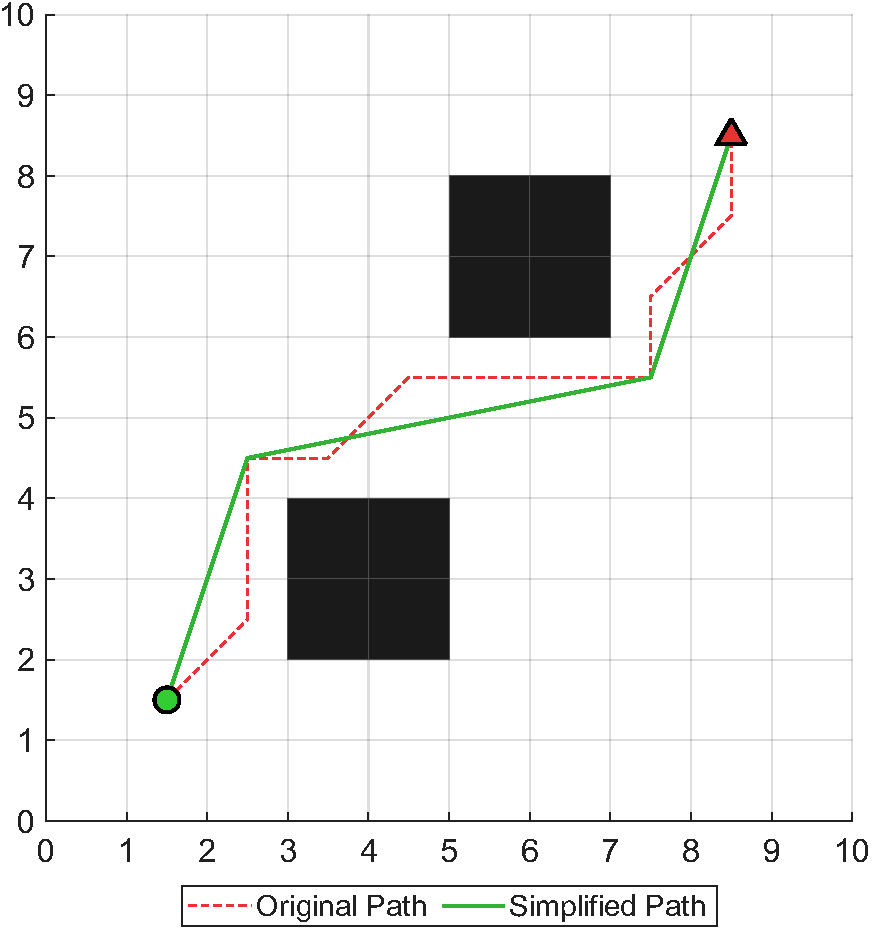
\includegraphics[width=1.55in]{figures/SimplifyPath}%
\label{fig:pipeline_a}}%
\hfil
\subfloat[Simplified path and smoothed path]{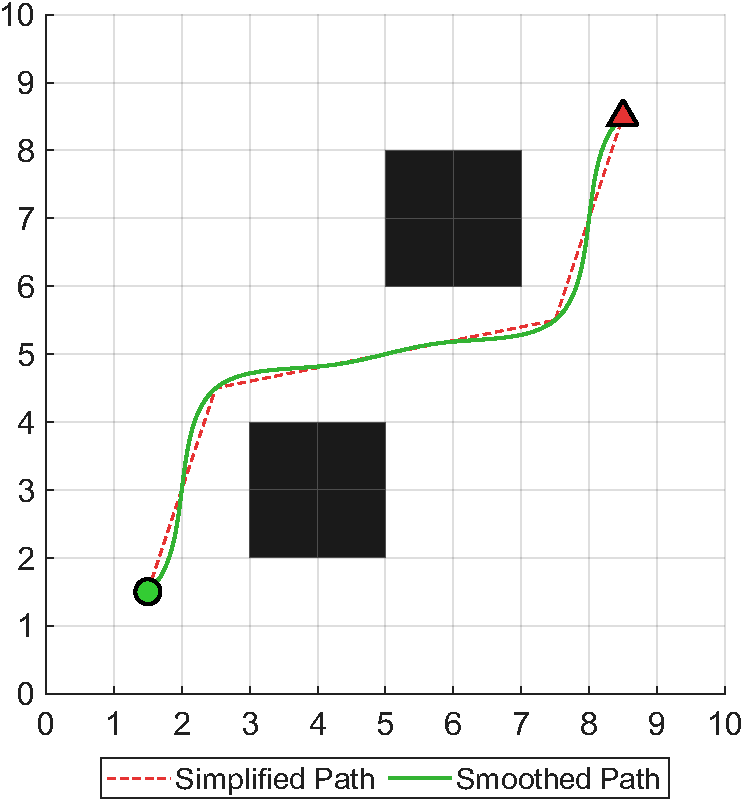
\includegraphics[width=1.55in]{figures/SmoothPath}%
\label{fig:pipeline_b}}
\caption{Comparison of the path at the individual stages of the pipeline.}
\label{fig:pipeline}
\end{figure}
